\documentclass[pdf]{beamer}
\setbeamertemplate{footline}[frame number]
\setbeamertemplate{section in toc}[sections numbered]
\usepackage{graphicx}
\mode<presentation>{
    \setbeamertemplate{page number in head/foot}[appendixframenumber]
}

\title{The Chinese Head Tax and Chinese Immigration to Canada}
\author{Amy Kim}
\date{October 11, 2022}

\begin{document}
\begin{frame}
    \titlepage
\end{frame}

\begin{frame}{Research Question}
    How did the Chinese Head Tax affect selection into immigration and/or immigrant wealth of Chinese immigrants to Canada in the early 20th century?    
\end{frame}

\begin{frame}{Outline}
    \tableofcontents
\end{frame}

\AtBeginSection[ ]
{
\begin{frame}{Outline}
    \tableofcontents[currentsection]
\end{frame}
}

% BACKGROUND
\section{Background}
\begin{frame}{Timeline}
    \begin{itemize}
        \item Early 1880s: Influx of Chinese immigrants for construction of Canadian Pacific Railway
        \item 1885: Chinese Exclusion Act institutes \$50 tax
        \begin{itemize}
            \item Only exceptions for students, merchants, and diplomats
            \item Was not applied retroactively, but the tax was required even for re-entry going forward
            \item One-time tax\footnote{Repayment was only required if someone was out of the country for more than 2 years}, applied at the port of entry
            \item Payment was tracked using a physical `head-tax certificate'
            \item Failure to pay would result in being sent back to China -- many immigrants had to borrow money or enter indentured servitude contracts
        \end{itemize}
    \end{itemize}
\end{frame}

\begin{frame}{Timeline}
    \begin{itemize}
        \item 1900: Tax raised to \$100 
        \item 1903: Tax raised to \$500 
        \item 1912: All certificates re-issued with a photo (to prevent entry using someone else's certificate)
        \item 1923: Chinese immigration banned completely (with very few exceptions)
        \item Chan (2014) estimates that the Canadian government generated \$23 million in revenue from the Head Tax (approx. 440 million USD today)
    \end{itemize}
\end{frame}

% DATA
\section{Data}
\subsection{Census Data}
\begin{frame}{Canadian Census Data}
    \centering
    \begin{tabular}{|r||c|c|}
        \hline 
        Year & Coverage & Sampling Method \\
        \hline 
        1852 & 20\% & Random, clustered sample \\
        1871 & 1.8\% & Stratified sample (8 strata)\\
        1881 & 100\% & Full sample \\
        1891 & 5\% & Random sample\footnote{Also includes 10\% of cities and 100\% of all large dwellings and some areas of Ontario} \\
        1901 & 5\% & \textit{Not Specified} \\
        1911 & 5\% & Random sample\footnote{Also includes 10\% of large dwellings and 25\% of multi-unit dwellings} \\
        1921 & 4\% & Random sample\footnote{Also includes 10\% of large dwellings and 20\% of multi-unit dwellings} \\
        \hline
    \end{tabular} \\
    Note: China was not listed as a country of origin in the data until the 1881 census.
\end{frame}

\begin{frame}{Canadian Census Data}
    
\includegraphics[width = \textwidth]{../../figs/census_tweet.png}
\end{frame}

\subsection{Chinese Registry}
\begin{frame}{Chinese Registry Data}
    \centering
    \begin{itemize}
        \item Publicly available and fully digitized
        \item Includes a full count of every person of Chinese origin arriving in Canada from 1885-1949
        \item Also includes information on pre-1885 entrants who chose to register for re-entry 
        \item Includes: Name, Age, Sex, Occupation, Date \& Port of Arrival, \textbf{Fee paid}, Area of Origin in China, Date of Re-Entry (if applicable) 
    \end{itemize}
    \hyperlink{summstats}{\beamerbutton{Summary Statistics for Census vs Registry Data}} \\ 
    TODO : add t-test to the summ stats table 
\end{frame}



% INITIAL DESCRIPTIVES
\section{Initial Descriptives}
\subsection{Immigration in Response to Head Tax}
\begin{frame}[label = yrimmchi]{Chinese Immigration to Canada by Year and Data Source}
    \centering
    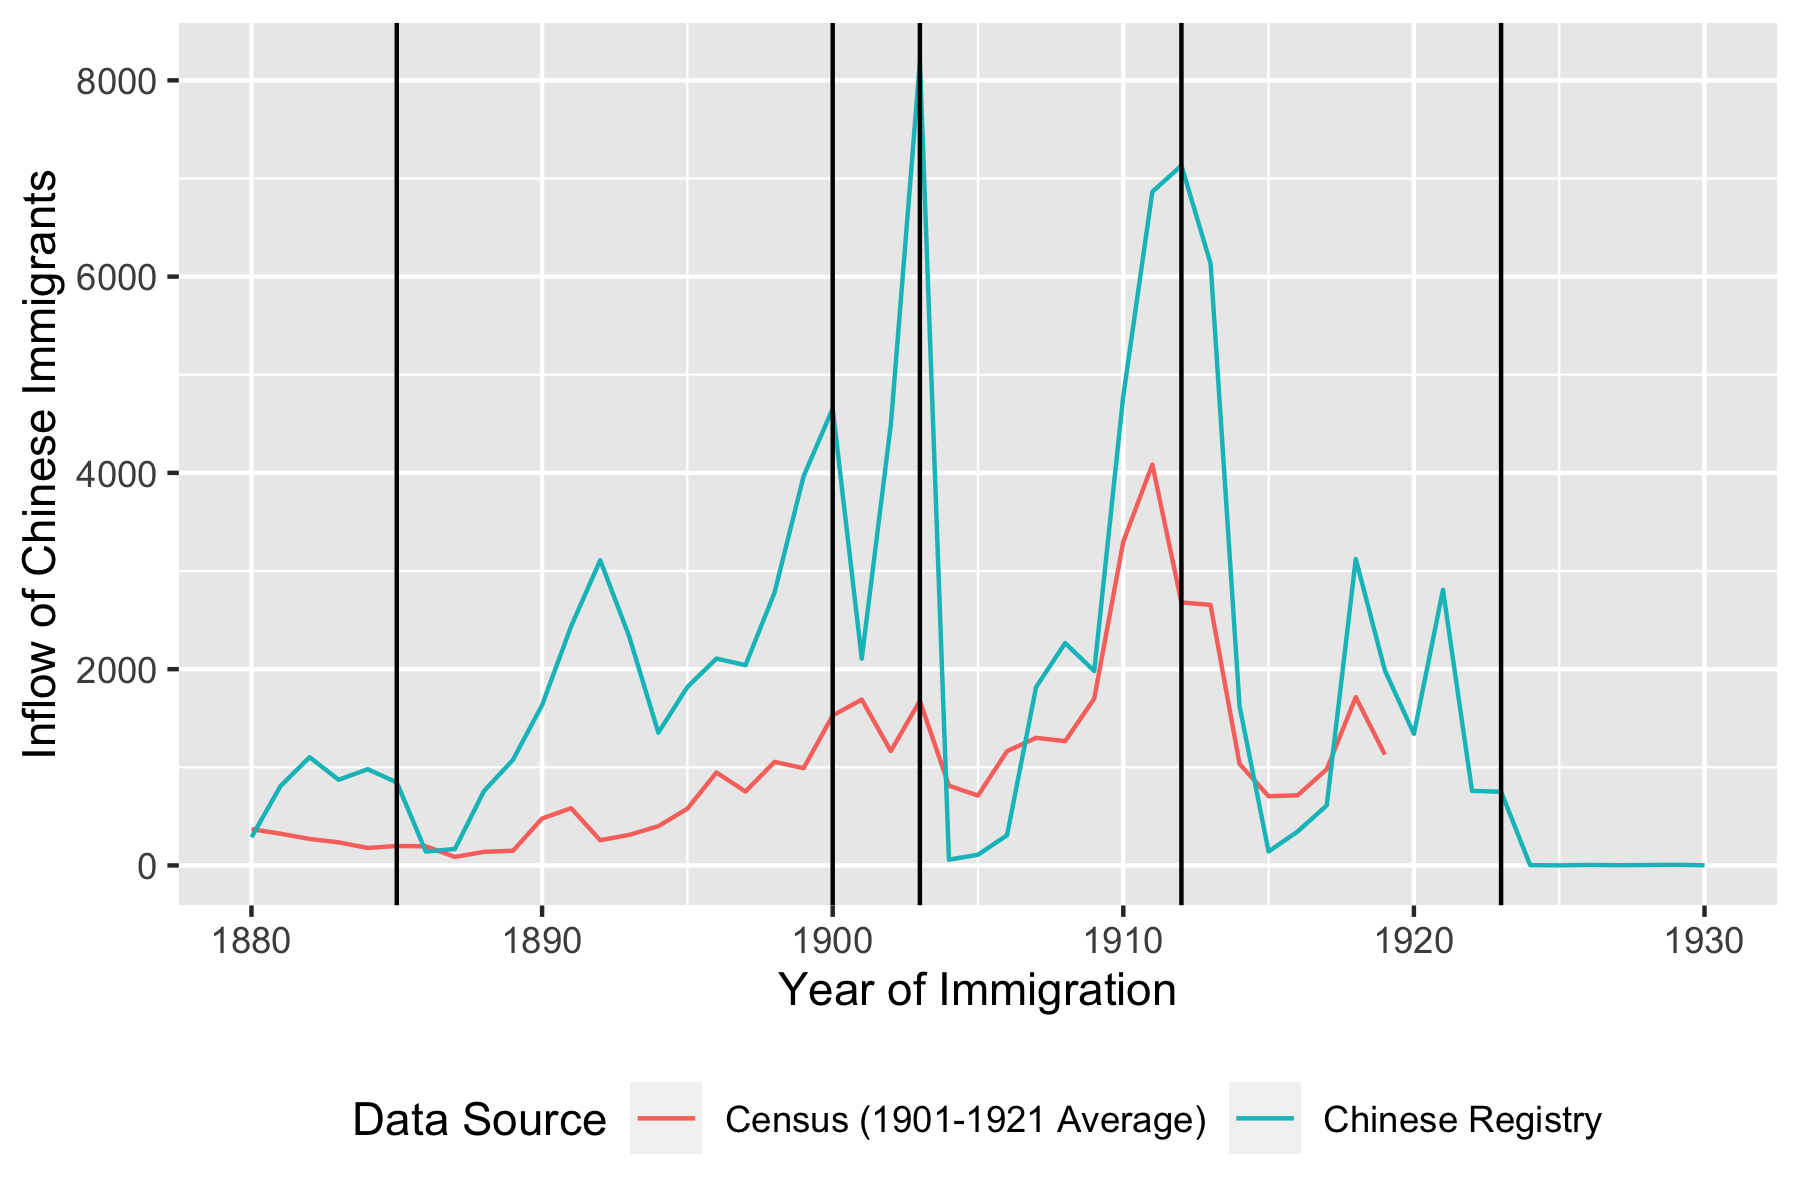
\includegraphics[width = 0.9\textwidth]{../../figs/yrimmchi.png}
    \hyperlink{dateimmchi}{\beamerbutton{Denisty of Chinese Immigration by Date}}
\end{frame}

\begin{frame}[label = events1912]
	\frametitle{Relevant Events in the 1910s}
	\begin{itemize}
        \item Canada: Head Tax Certificates reissued with photo 
        \begin{itemize}
            \item Unlikely to have such a massive spike just from using other people's certificates 
        \end{itemize}
        \item China: Republic of China established in 1912 following Xinhai Revolution (1911)
        \begin{itemize}
            \item If this is primary cause of spike, would expect some change in regional origin of Chinese immigrants \hyperlink{originchi}{\beamerbutton{Chinese Immigration by Origin by Year}}
            \item Also would not expect to see spike in immigration from other countries \hyperlink{yrimmall}{\beamerbutton{Immigration to Canada from Different Countries}}
        \end{itemize}
        \item Worldwide: WWI begins July 1914
        \begin{itemize}
            \item Unclear why most of spike is prior to 1914 -- general global unrest?
        \end{itemize}
    \end{itemize}
\end{frame}

\begin{frame}[label = yrimmall]
	\frametitle{Immigration to Canada by Year by Country}
    \centering
	\begin{figure}[H]
		\begin{center}
			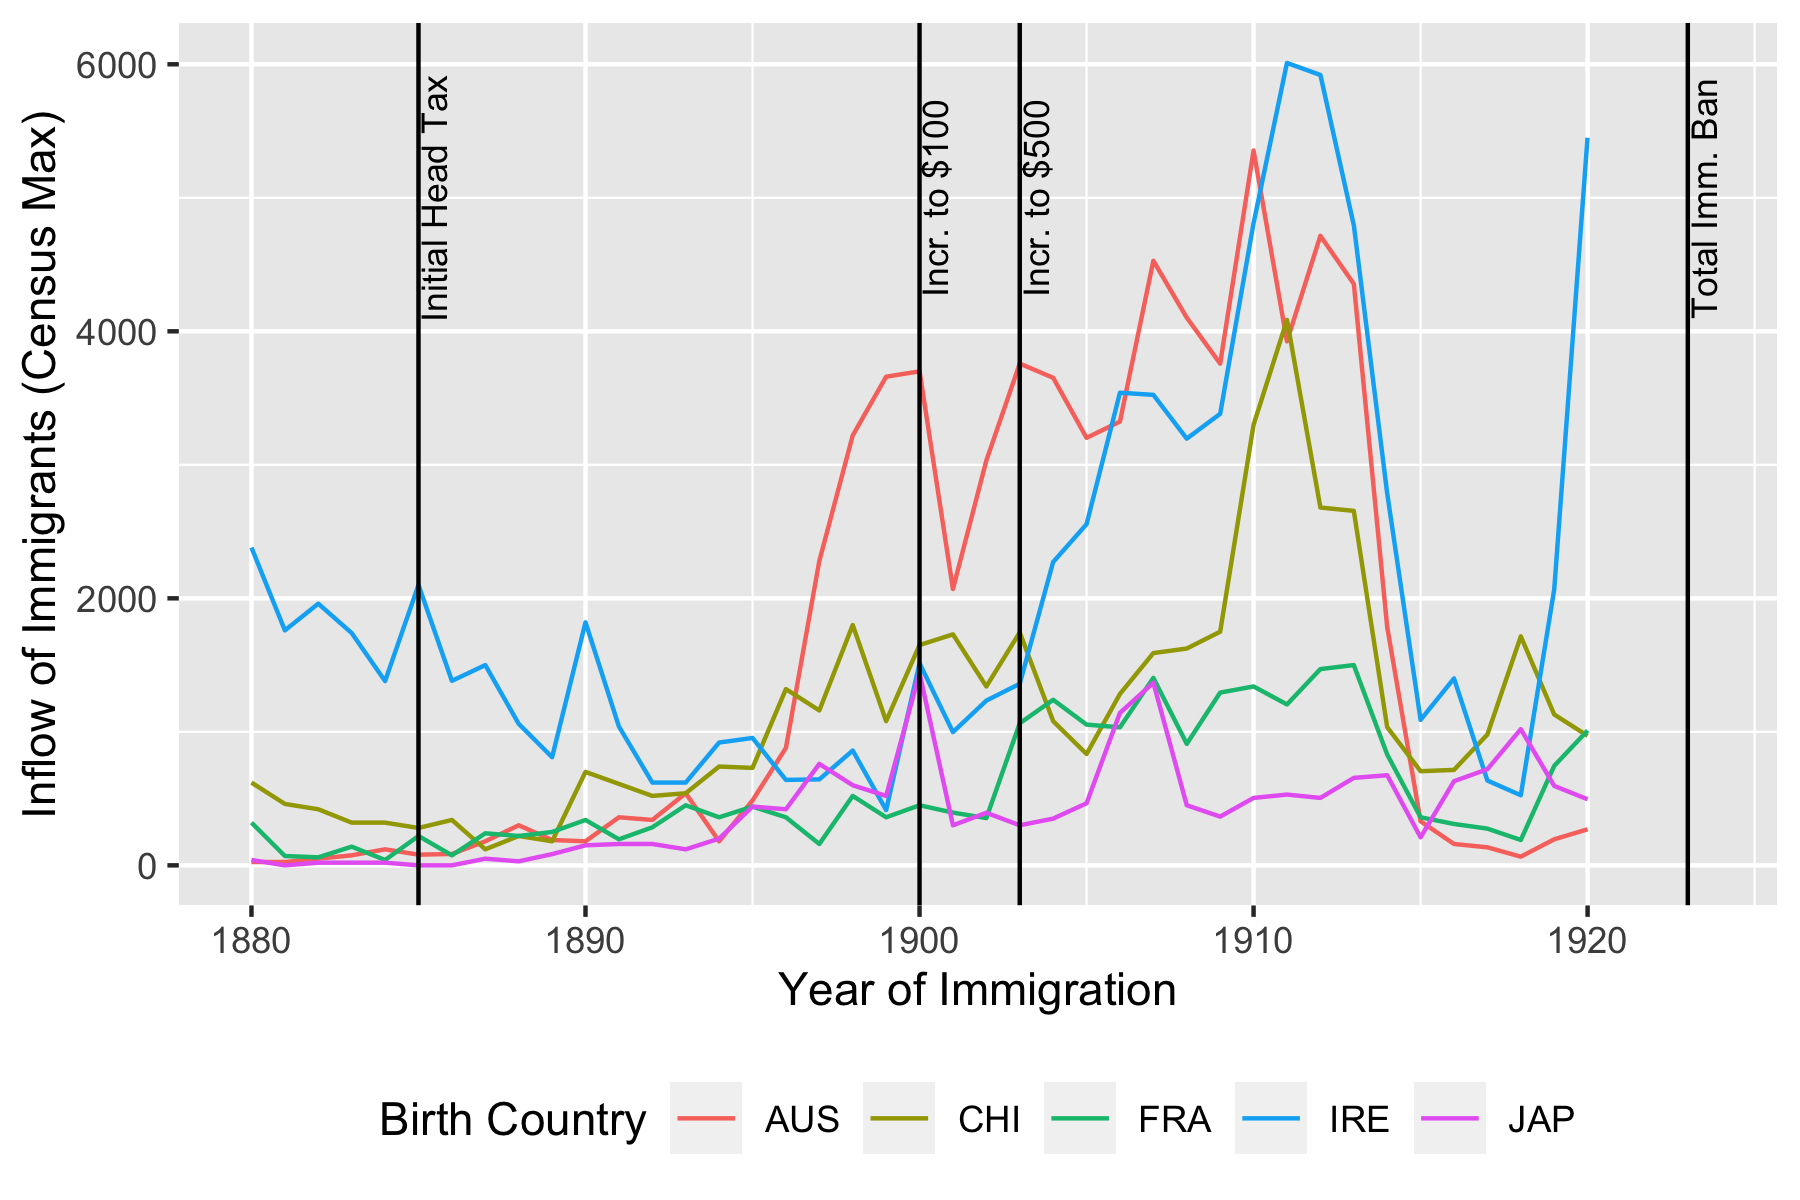
\includegraphics[width=\textwidth]{../../figs/yrimmall.png}
		\end{center}
	\end{figure}
\end{frame}

\begin{frame}{Head Tax Payers: Taxes Paid and Fraction of Arrivals}
    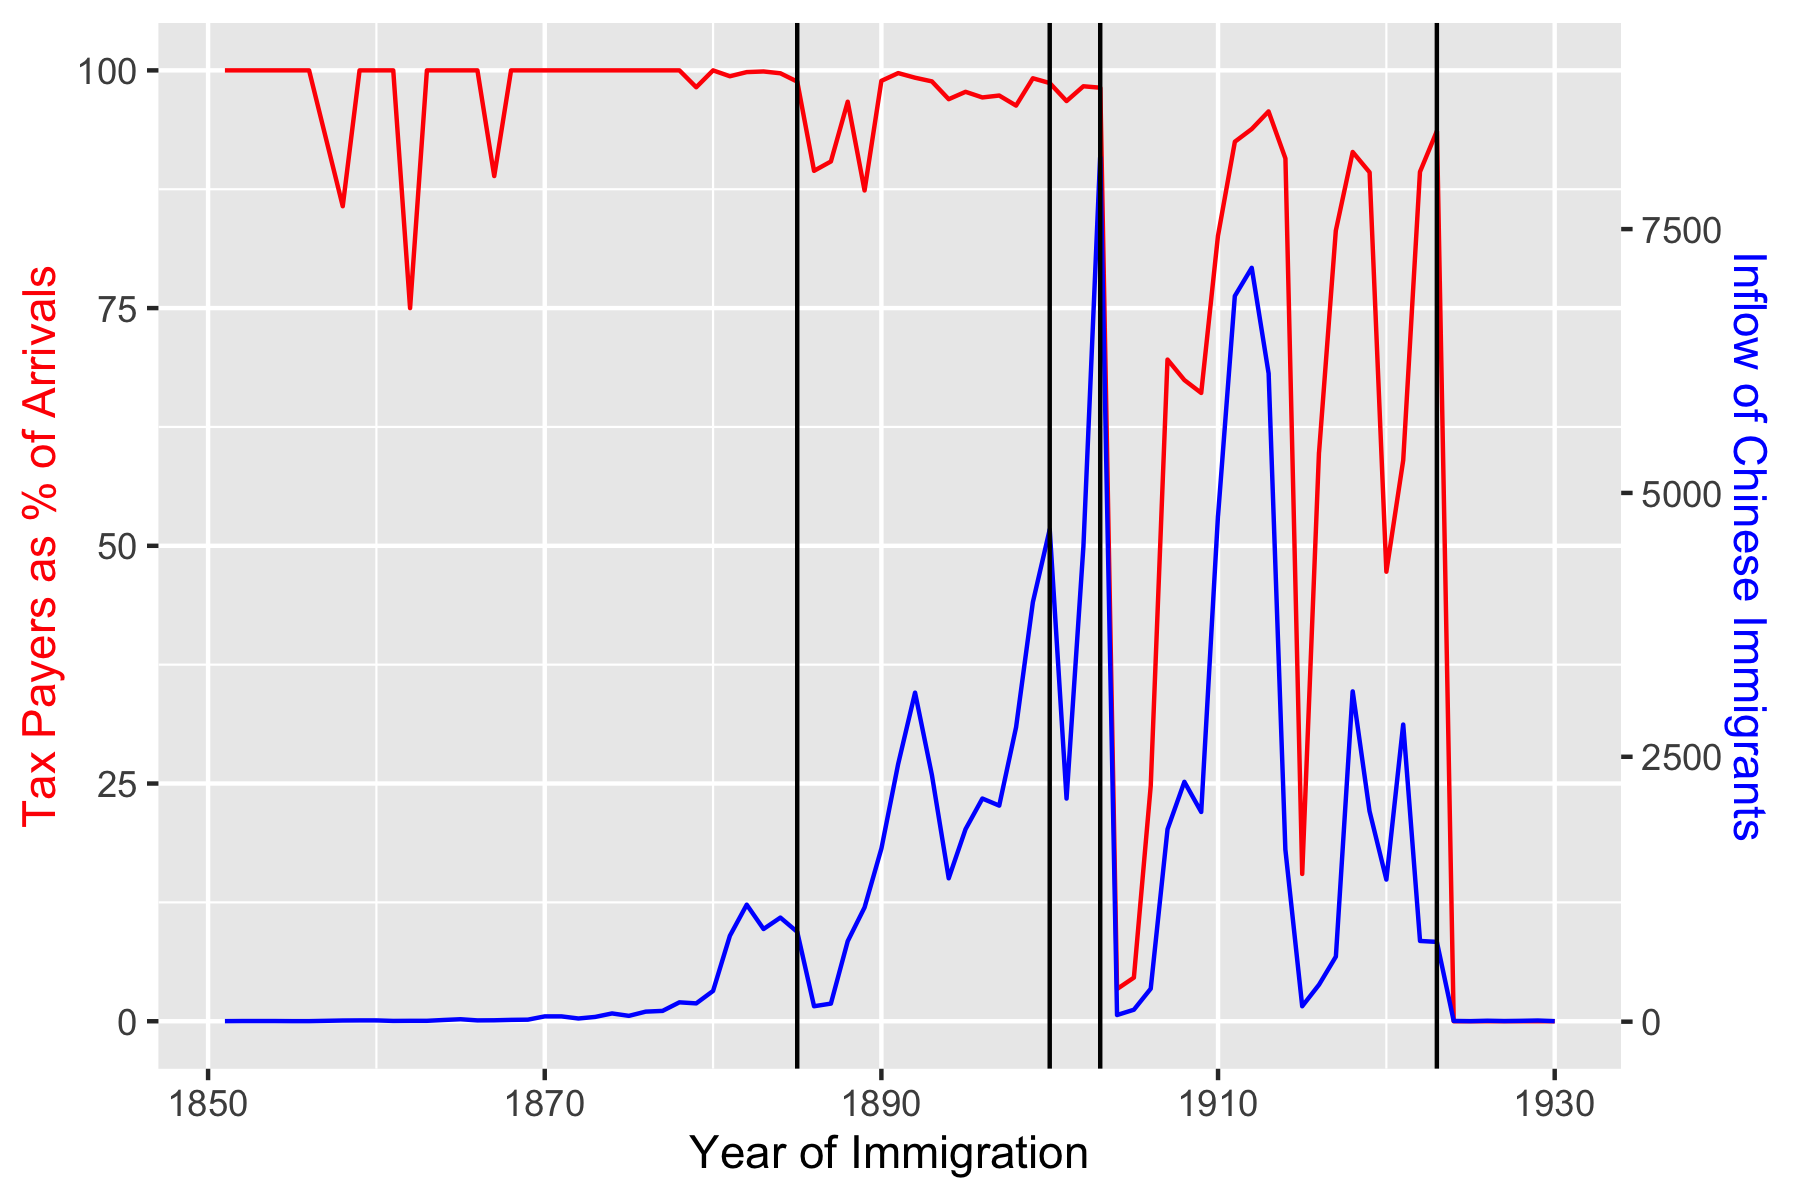
\includegraphics[width = \textwidth]{../../figs/taxbyyear.png}
\end{frame}

\subsection{Decomposing Chinese Immigration}
\begin{frame}{Chinese Immigration by Occupation Group}
    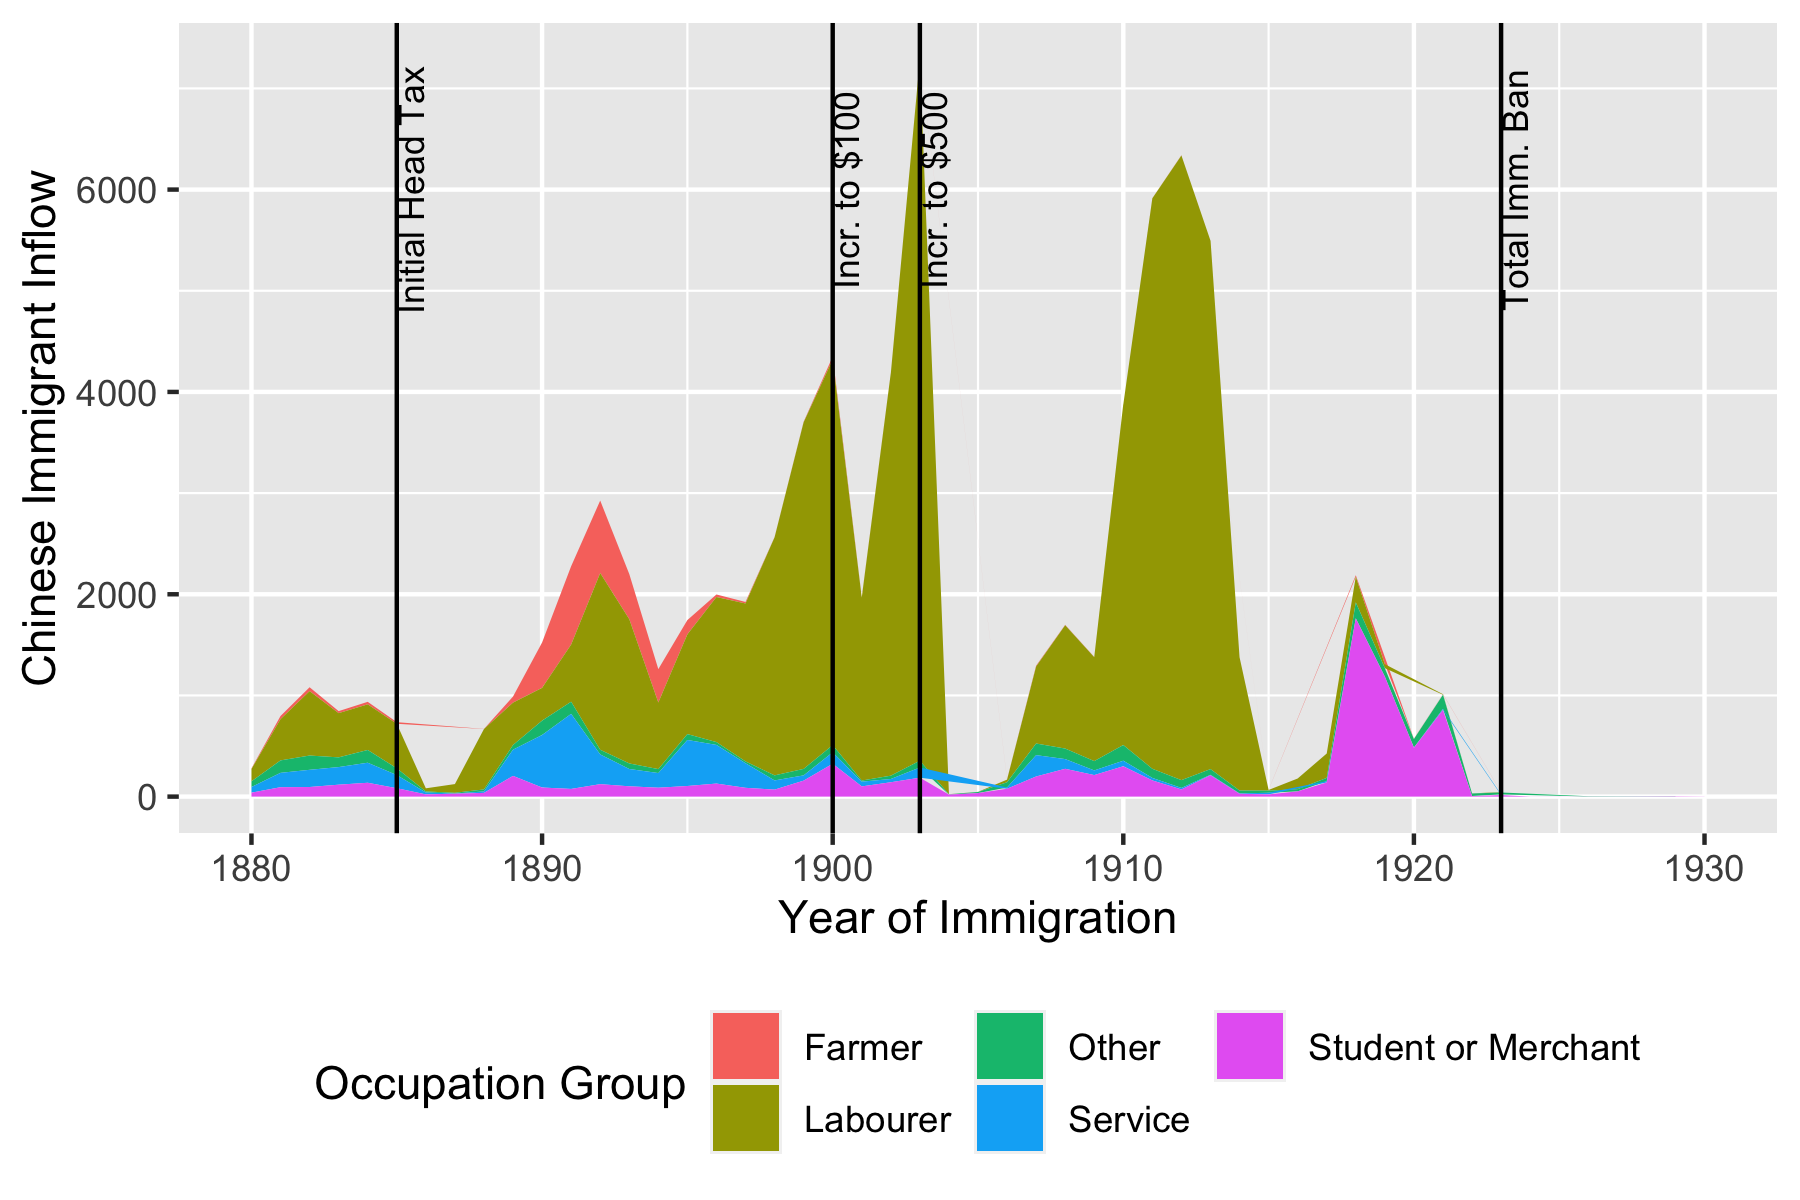
\includegraphics[width = \textwidth]{../../figs/chiocc.png}
\end{frame}

%%%%%%%%%%%%%%%%%%%%%%%%%%%%%%%%%%%%%%%%%%%%%%%%%%%%%%%
%%%%%%%%%%      A  P  P  E  N  D  I  X      %%%%%%%%%%%
%%%%%%%%%%%%%%%%%%%%%%%%%%%%%%%%%%%%%%%%%%%%%%%%%%%%%%%
\appendix
%---------------------------
%   Summary Statistics for Census vs Registry Data
%---------------------------
\begin{frame}[label = summstats]
	\frametitle{Summary Statistics}
	\begin{table}[H]
        \centering 
		\resizebox{\textwidth}{!}{
            % latex table generated in R 4.0.3 by xtable 1.8-4 package
% Mon Oct 10 23:48:19 2022
\begin{tabular}{lccc}
  \hline
 & CA Census (1901-1921) & Chinese Registry (1885-1924) & US Census (1900-1920) \\ 
  \hline
\% Male & 0.98 & 0.98 & 0.95 \\ 
   & (0.16) & (0.15) & (0.21) \\ 
  \% Married & 0.55 & - & 0.44 \\ 
    & (0.5) & - & (0.5) \\ 
  Avg. Age at Imm & 23.20 & 25.95 & 20.92 \\ 
     & (8.99) & (21.86) & (9.78) \\ 
  \% Can Read & 0.68 & - & 0.77 \\ 
        & (0.47) & - & (0.42) \\ 
  \% Labourers & 0.20 & 0.62 & 0.32 \\ 
           & (0.4) & (0.48) & (0.47) \\ 
   \hline
Obs &   4230 &  90946 & 186523 \\ 
   \hline
\end{tabular}

		}
	\end{table}  
\end{frame}

%---------------------------
%   Density of Chinese Immigration to Canada by Date
%---------------------------

\begin{frame}[label = dateimmchi]
	\frametitle{Density of Chinese Immigration to Canada by Date}
    \centering
	\begin{figure}[H]
		\begin{center}
			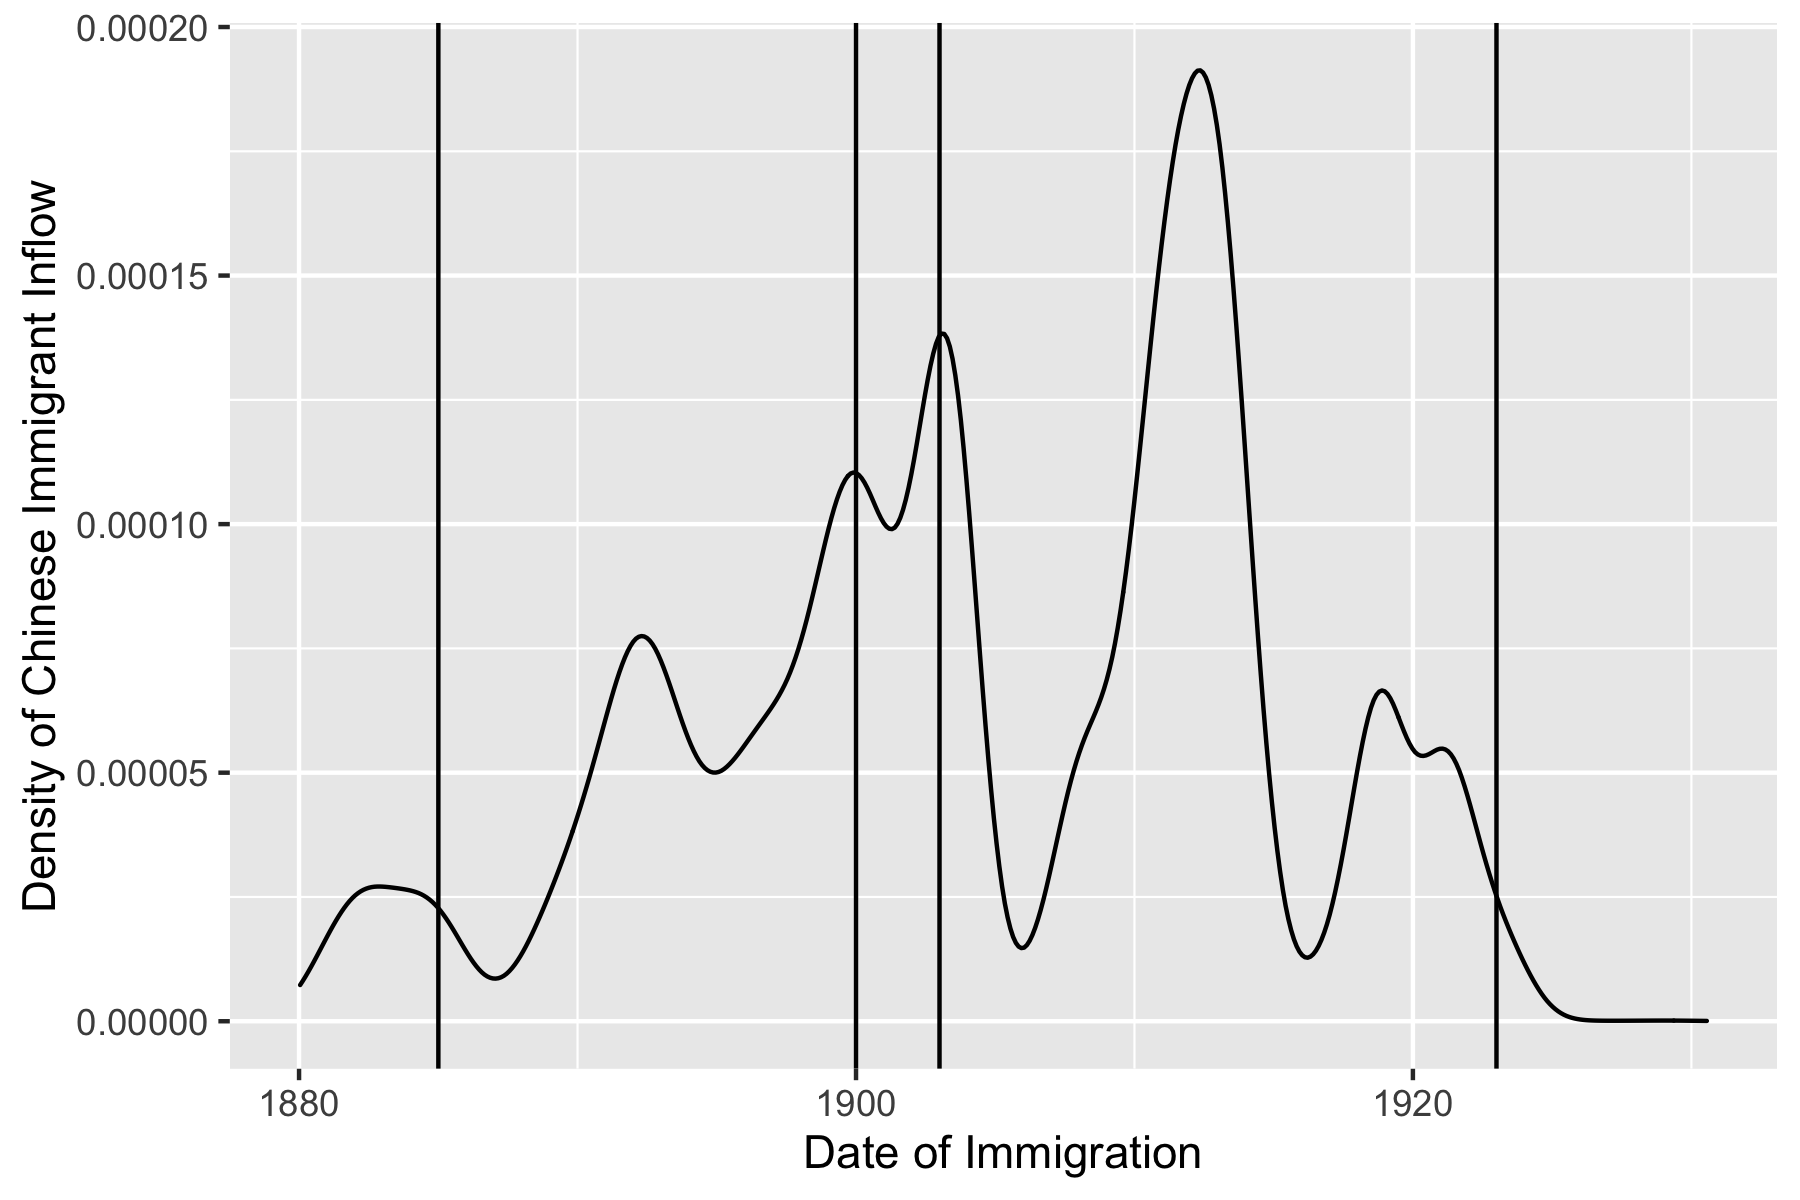
\includegraphics[width=\textwidth]{../../figs/dateimmchi.png}
		\end{center}
	\end{figure}
    \hyperlink{yrimmchi}{\beamerbutton{Back to Slides}}
\end{frame}

%---------------------------
%   Chinese immigration by Origin County
%---------------------------
\begin{frame}[label = originchi]
	\frametitle{Chinese Immigration by County of Origin in China}
    \centering
	\begin{figure}[H]
		\begin{center}
			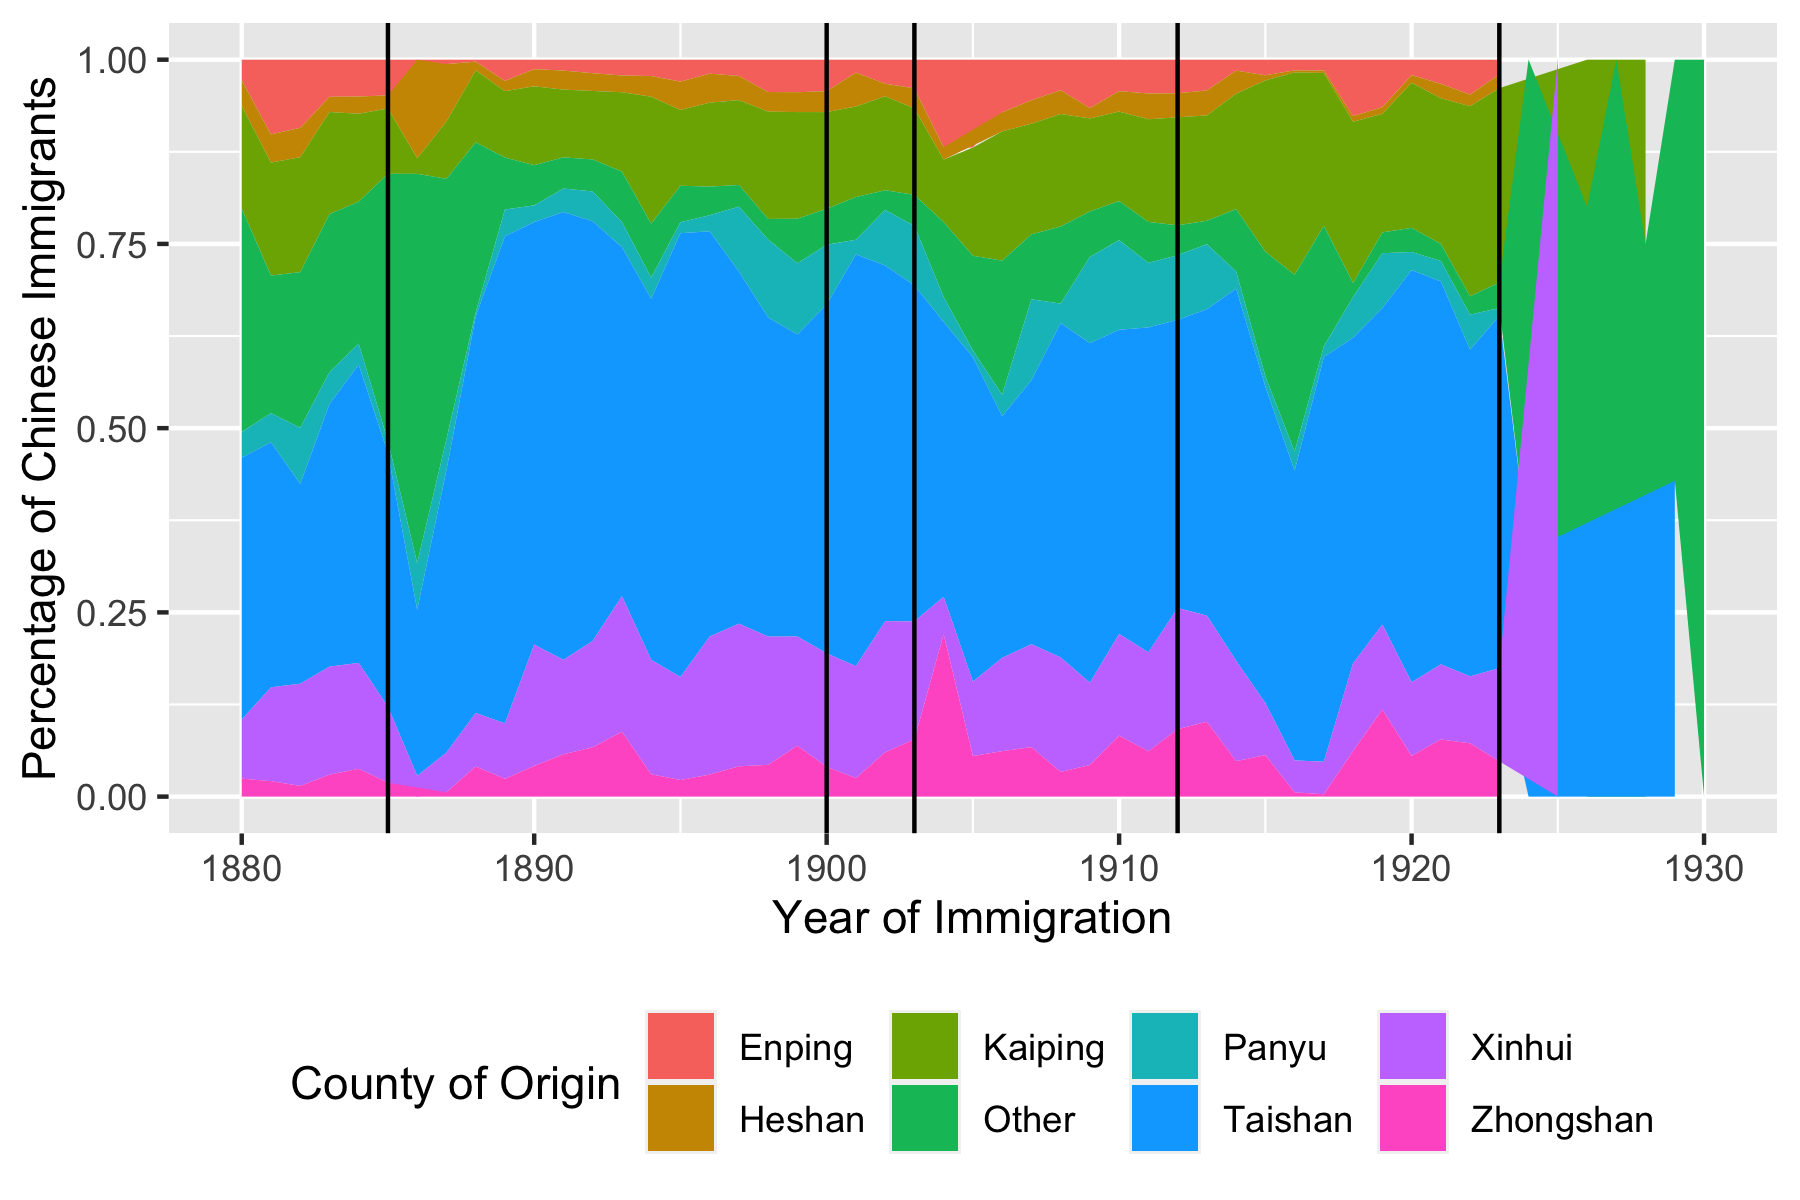
\includegraphics[width=\textwidth]{../../figs/chiorig.png}
		\end{center}
	\end{figure}
    \hyperlink{events1912}{\beamerbutton{Back to Slides}}
\end{frame}

\end{document}